\batchmode

\documentclass{article}
\makeatletter

\usepackage{html}

  

 

\usepackage{makeidx,graphicx}
\usepackage{natbib}

\usepackage{rcs,fancyheadings}
\usepackage{nummargins}

\pagestyle{fancy} 
\RCS $RCSfile: images.tex,v $
\RCS $Revision: 1.1.1.1 $
\RCS $Date: 2002/01/02 19:36:48 $
\lhead{\RCSRCSfile} 
\rhead{Lab two: page~\thepage} 
\chead{\RCSRevision}
\lfoot{}
\cfoot{}
\rfoot{}

\title{Laboratory \#2:\\  An Introduction to the Numerical Solution of
  Differential Equations: \\  Discretization, accuracy and stability
}
\author{John M. Stockie}
\date{Date printed: \today}

\makeindex
\makeglossary

\newcommand{\labnumber}{2}

\newcommand{\imageURL}[1]{http://www.geog.ubc.ca/numeric/labs/lab2/images/#1}

\newcommand{\cgibinURL}[1]{http://www.geog.ubc.ca/numeric/labs/lab2/cgi-bin/#1}

\newcommand{\quizURL}[1]{http://www.geog.ubc.ca/numeric/labs/cgi-bin/tutorial.cgi//numeric/labs/lab2/quiz/#1}

\newcommand{\SourceDir}{http://www.geog.ubc.ca/numeric/labs/lab2/source/}

\newcommand{\SourceFile}[1]{http://www.geog.ubc.ca/numeric/labs/lab2/source/#1}

\newcommand{\latextwoe}{\mbox{\textbf{\LaTeX-2e}}}

\newcommand{\BibFile}{/home/numeric/refs}

\newcommand{\psbutton}[1]{/nfs/dragon/local1/www/numeric/psbutton/#1}

\newcommand{\buttonURL}[1]{http://www.geog.ubc.ca/numeric/AIcons/Buttons/#1}

\newcommand{\quiz}[2]{
\htmladdnormallinkfoot{\htmladdimg{\buttonURL{question.gif}} #2}{\quizURL{#1}} 
}

\newcommand{\demo}[2]{
\htmladdnormallinkfoot{\htmladdimg{\buttonURL{eye.gif}} #2}{\cgibinURL{#1}} 
}

\newcommand{\movie}[2]{
\htmladdnormallinkfoot{\htmladdimg{\buttonURL{film.gif}} #2}{\imageURL{#1}} 
}

\newcommand{\technicalnote}[4]{
  \hyperref{\htmladdimg{http://www.geog.ubc.ca/numeric/images/computer3.gif}\ #1}{
\includegraphics[scale=0.65]{\psbutton{computer3.eps}} #2}{#3}{#4}
}

\newcounter{example}

\renewcommand{\theexample}{\arabic{example}}

\newcounter{problem}

\renewcommand{\theproblem}{\arabic{problem}}

\newenvironment{note}
{\begin{quote}{\htmladdimg{http://www.geog.ubc.ca/numeric/images/note.gif}
      \textbf{Note:}}}
  {\end{quote}}

\newenvironment{mathnote}
{\begin{quote}{\htmladdimg{http://www.geog.ubc.ca/numeric/images/math3.gif}
      \textbf{Mathematical Note:}}}
  {\end{quote}}

\newcommand{\gloss}[2]{\glossary{#1::#2}}

\renewcommand{\theequation}{\thesection.\arabic{equation}}

\newcommand{\LaboneURL}{http://www.eos.ubc.ca/numeric/labs/lab1/lab1.pdf}

\newcommand{\LabtwoURL}{http://www.eos.ubc.ca/numeric/labs/lab2/lab2.pdf}

\newcommand{\LabthreeURL}{http://www.eos.ubc.ca/numeric/labs/lab3/lab3.pdf}

\newcommand{\LabfourURL}{http://www.eos.ubc.ca/numeric/labs/lab4/lab4.pdf}

\newcommand{\LabfiveURL}{http://www.eos.ubc.ca/numeric/labs/lab5/lab5.pdf}

\newcommand{\LabsixURL}{http://www.eos.ubc.ca/numeric/labs/lab6/lab6.pdf}

\newcommand{\LabsevenURL}{http://www.eos.ubc.ca/numeric/labs/lab7/lab7.pdf}

\newcommand{\LabeightURL}{http://www.eos.ubc.ca/numeric/labs/lab8/lab8.pdf}

\newcommand{\LabXsURL}{http://www.eos.ubc.ca/numeric/labs/labX/labX/labX.html}

\newcommand{\LabsURL}[1]{http://www.eos.ubc.ca/numeric/labs/#1}

\newcommand{\OctaveHelpLink}{\externalref{lab3:sec:oct}}

\newcommand{\ie}{i.e.~}

\newcommand{\eg}{e.g.~}

\newcommand{\dt}{\mbox{$\Delta t$}{}}

\newcommand{\yi}{\mbox{$y_i$}{}}

\newcommand{\ti}{\mbox{$t_i$}{}}

\newcommand{\eqref}[1]{(\ref{#1})}

\AtBeginDocument{\input /amd/peacock/root/local1/homes/numeric/labs/lab2/lab2.aux }
\makeatother
\ifx\AtBeginDocument\undefined \newcommand{\AtBeginDocument}[1]{}\fi
\newenvironment{tex2html_wrap}{}{}
\newbox\sizebox
\setlength{\hoffset}{0pt}\setlength{\voffset}{0pt}
\addtolength{\textheight}{\footskip}\setlength{\footskip}{0pt}
\addtolength{\textheight}{\topmargin}\setlength{\topmargin}{0pt}
\addtolength{\textheight}{\headheight}\setlength{\headheight}{0pt}
\addtolength{\textheight}{\headsep}\setlength{\headsep}{0pt}
\setlength{\textwidth}{451pt}
\newwrite\lthtmlwrite
\makeatletter
\let\realnormalsize=\normalsize
\topskip=0pt
\def\preveqno{}\let\real@float=\@float \let\realend@float=\end@float
\def\@float{\let\@savefreelist\@freelist\real@float}
\def\end@float{\realend@float\global\let\@freelist\@savefreelist}
\let\real@dbflt=\@dbflt \let\end@dblfloat=\end@float
\let\@largefloatcheck=\relax
\def\@dbflt{\let\@savefreelist\@freelist\real@dbflt}
\def\adjustnormalsize{\def\normalsize{\mathsurround=0pt \realnormalsize\parindent=0pt\abovedisplayskip=0pt\belowdisplayskip=0pt}\normalsize}
\def\lthtmltypeout#1{{\let\protect\string\immediate\write\lthtmlwrite{#1}}}%
\newcommand\lthtmlhboxmathA{\adjustnormalsize\setbox\sizebox=\hbox\bgroup}%
\newcommand\lthtmlvboxmathA{\adjustnormalsize\setbox\sizebox=\vbox\bgroup%
 \let\ifinner=\iffalse }%
\newcommand\lthtmlboxmathZ{\@next\next\@currlist{}{\def\next{\voidb@x}}%
 \expandafter\box\next\egroup}%
\newcommand\lthtmlmathtype[1]{\def\lthtmlmathenv{#1}}%
\newcommand\lthtmllogmath{\lthtmltypeout{l2hSize %
:\lthtmlmathenv:\the\ht\sizebox::\the\dp\sizebox::\the\wd\sizebox.\preveqno}}%
\newcommand\lthtmlfigureA[1]{\let\@savefreelist\@freelist
       \lthtmlmathtype{#1}\lthtmlvboxmathA}%
\newcommand\lthtmlfigureZ{\lthtmlboxmathZ\lthtmllogmath\copy\sizebox
       \global\let\@freelist\@savefreelist}%
\newcommand\lthtmldisplayA[1]{\lthtmlmathtype{#1}\lthtmlvboxmathA}%
\newcommand\lthtmldisplayB[1]{\edef\preveqno{(\theequation)}%
  \lthtmldisplayA{#1}\let\@eqnnum\relax}%
\newcommand\lthtmldisplayZ{\lthtmlboxmathZ\lthtmllogmath\lthtmlsetmath}%
\newcommand\lthtmlinlinemathA[1]{\lthtmlmathtype{#1}\lthtmlhboxmathA  \vrule height1.5ex width0pt }%
\newcommand\lthtmlinlinemathZ{\egroup\expandafter\ifdim\dp\sizebox>0pt %
  \expandafter\centerinlinemath\fi\lthtmllogmath\lthtmlsetmath}
\def\lthtmlsetmath{\hbox{\vrule width.5pt\vtop{\vbox{%
  \kern.5pt\kern1.25 pt\hbox{\hglue.5pt\copy\sizebox\hglue1.25 pt}\kern.5pt%
  \ifdim\dp\sizebox>0pt\kern1.25 pt\fi}%
  \ifdim\hsize>\wd\sizebox \hrule depth1pt\fi}}}
\def\centerinlinemath{\dimen1=\ht\sizebox
  \ifdim\dimen1<\dp\sizebox \ht\sizebox=\dp\sizebox
  \else \dp\sizebox=\ht\sizebox \fi}

\def\lthtmlcheckvsize{\ifdim\ht\sizebox<\vsize\expandafter\vfill
  \else\expandafter\vss\fi}%
\makeatletter


\begin{document}
\pagestyle{empty}\thispagestyle{empty}%
\lthtmltypeout{latex2htmlLength hsize=\the\hsize}%
\lthtmltypeout{latex2htmlLength vsize=\the\vsize}%
\lthtmltypeout{latex2htmlLength hoffset=\the\hoffset}%
\lthtmltypeout{latex2htmlLength voffset=\the\voffset}%
\lthtmltypeout{latex2htmlLength topmargin=\the\topmargin}%
\lthtmltypeout{latex2htmlLength topskip=\the\topskip}%
\lthtmltypeout{latex2htmlLength headheight=\the\headheight}%
\lthtmltypeout{latex2htmlLength headsep=\the\headsep}%
\lthtmltypeout{latex2htmlLength parskip=\the\parskip}%
\lthtmltypeout{latex2htmlLength oddsidemargin=\the\oddsidemargin}%
\makeatletter
\if@twoside\lthtmltypeout{latex2htmlLength evensidemargin=\the\evensidemargin}%
\else\lthtmltypeout{latex2htmlLength evensidemargin=\the\oddsidemargin}\fi%
\makeatother
\stepcounter{section}
\stepcounter{section}
\stepcounter{section}
{\newpage\clearpage
\lthtmlinlinemathA{tex2html_wrap_inline243}%
$T^\prime(t)$%
\lthtmlinlinemathZ
\hfill\lthtmlcheckvsize\clearpage}

{\newpage\clearpage
\lthtmlinlinemathA{tex2html_wrap_inline247}%
$t_i=t_0+i \Delta t$%
\lthtmlinlinemathZ
\hfill\lthtmlcheckvsize\clearpage}

{\newpage\clearpage
\lthtmlinlinemathA{tex2html_wrap_inline249}%
$i
= 0,1,\ldots, N$%
\lthtmlinlinemathZ
\hfill\lthtmlcheckvsize\clearpage}

{\newpage\clearpage
\lthtmlinlinemathA{tex2html_wrap_inline251}%
$\Delta t= 1/N$%
\lthtmlinlinemathZ
\hfill\lthtmlcheckvsize\clearpage}

{\newpage\clearpage
\lthtmldisplayA{displaymath209}%
\begin{displaymath}T^\prime(t_i) \approx \frac{T_{i+1}-T_i}{\Delta t},
  \end{displaymath}%
\lthtmldisplayZ
\hfill\lthtmlcheckvsize\clearpage}

{\newpage\clearpage
\lthtmldisplayA{displaymath215}%
\begin{displaymath}T^\prime(t_i) \approx \frac{T_{i}-T_{i-1}}{\Delta t},
  \end{displaymath}%
\lthtmldisplayZ
\hfill\lthtmlcheckvsize\clearpage}

{\newpage\clearpage
\lthtmldisplayA{displaymath222}%
\begin{displaymath}T^\prime(t_i) \approx \frac{T_{i+1}-T_{i-1}}{2 \Delta t}.
  \end{displaymath}%
\lthtmldisplayZ
\hfill\lthtmlcheckvsize\clearpage}

{\newpage\clearpage
\lthtmlinlinemathA{tex2html_wrap_inline253}%
$\Delta t$%
\lthtmlinlinemathZ
\hfill\lthtmlcheckvsize\clearpage}

\stepcounter{section}
\refstepcounter{example}
{\newpage\clearpage
\lthtmldisplayA{displaymath265}%
\begin{displaymath}\frac{dT}{dt} = \lambda(T,t) \, (T-T_a) 
  \end{displaymath}%
\lthtmldisplayZ
\hfill\lthtmlcheckvsize\clearpage}

{\newpage\clearpage
\lthtmldisplayA{displaymath604}%
\begin{displaymath}T_{i+1} = T_i + \Delta t \, \lambda(T_i,t_i) \, (T_i-T_a).
  \end{displaymath}%
\lthtmldisplayZ
\hfill\lthtmlcheckvsize\clearpage}

{\newpage\clearpage
\lthtmldisplayA{displaymath605}%
\begin{displaymath}T_{i+1} = T_i + \Delta t \, \lambda(T_{i+1},t_{i+1}) \, (T_{i+1}-T_a), 
  \end{displaymath}%
\lthtmldisplayZ
\hfill\lthtmlcheckvsize\clearpage}

{\newpage\clearpage
\lthtmldisplayA{displaymath606}%
\begin{displaymath}T_{i+1} = T_{i-1} + 2 \Delta t \, \lambda(T_{i},t_{i}) \, (T_{i}-T_a). 
  \end{displaymath}%
\lthtmldisplayZ
\hfill\lthtmlcheckvsize\clearpage}

{\newpage\clearpage
\lthtmlinlinemathA{tex2html_wrap_inline628}%
$\lambda$%
\lthtmlinlinemathZ
\hfill\lthtmlcheckvsize\clearpage}

{\newpage\clearpage
\lthtmlinlinemathA{tex2html_wrap_inline638}%
$\lambda=-0.8$%
\lthtmlinlinemathZ
\hfill\lthtmlcheckvsize\clearpage}

{\newpage\clearpage
\lthtmlinlinemathA{tex2html_wrap_inline646}%
$\Delta t=\frac{1}{3}$%
\lthtmlinlinemathZ
\hfill\lthtmlcheckvsize\clearpage}

{\newpage\clearpage
\lthtmlfigureA{figure292}%
\begin{figure}
    \begin{center}
      \leavevmode
      
\includegraphics [height=3.5in]{accuracy/compare1.eps}
    \end{center}
  \end{figure}%
\lthtmlfigureZ
\hfill\lthtmlcheckvsize\clearpage}

\stepcounter{subsection}
\stepcounter{subsubsection}
\stepcounter{paragraph}
\refstepcounter{example}
{\newpage\clearpage
\lthtmlinlinemathA{tex2html_wrap_inline648}%
$\pi$%
\lthtmlinlinemathZ
\hfill\lthtmlcheckvsize\clearpage}

{\newpage\clearpage
\lthtmlinlinemathA{tex2html_wrap_inline650}%
$3.1415926535897932385\dots$%
\lthtmlinlinemathZ
\hfill\lthtmlcheckvsize\clearpage}

{\newpage\clearpage
\lthtmldisplayA{displaymath607}%
\begin{displaymath}\frac{\pi}{(\pi + 0.00000001)-\pi}. 
  \end{displaymath}%
\lthtmldisplayZ
\hfill\lthtmlcheckvsize\clearpage}

{\newpage\clearpage
\lthtmlinlinemathA{tex2html_wrap_inline656}%
$\pi+0.00000001$%
\lthtmlinlinemathZ
\hfill\lthtmlcheckvsize\clearpage}

{\newpage\clearpage
\lthtmlinlinemathA{tex2html_wrap_inline660}%
$\frac{1}{0}$%
\lthtmlinlinemathZ
\hfill\lthtmlcheckvsize\clearpage}

{\newpage\clearpage
\lthtmlinlinemathA{tex2html_wrap_inline662}%
$100000000\pi$%
\lthtmlinlinemathZ
\hfill\lthtmlcheckvsize\clearpage}

\stepcounter{paragraph}
{\newpage\clearpage
\lthtmldisplayA{displaymath608}%
\begin{displaymath}T(t_{i+1}) = T(t_i+\mbox{$\Delta t$}{}) = T(t_i) + (\Delta t) T^\prime(t_i) + 
  \frac{1}{2}(\Delta t)^2 T^{\prime\prime}(t_i) +\cdots,
\end{displaymath}%
\lthtmldisplayZ
\hfill\lthtmlcheckvsize\clearpage}

{\newpage\clearpage
\lthtmlinlinemathA{tex2html_wrap_inline678}%
$y = {\cal O}(\Delta t)$%
\lthtmlinlinemathZ
\hfill\lthtmlcheckvsize\clearpage}

{\newpage\clearpage
\lthtmlinlinemathA{tex2html_wrap_inline680}%
$y<c \cdot \Delta t$%
\lthtmlinlinemathZ
\hfill\lthtmlcheckvsize\clearpage}

{\newpage\clearpage
\lthtmlinlinemathA{tex2html_wrap_inline696}%
$\Delta t^2$%
\lthtmlinlinemathZ
\hfill\lthtmlcheckvsize\clearpage}

{\newpage\clearpage
\lthtmlfigureA{figure367}%
\begin{figure}
  \begin{center}
    \leavevmode
    \htmlimage{scale=1.5}
    
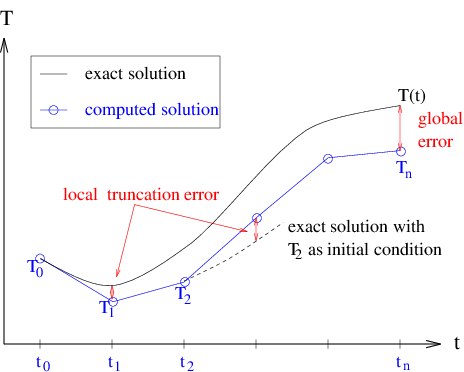
\includegraphics [height=3.0in]{images/error.eps}
  \end{center}
\end{figure}%
\lthtmlfigureZ
\hfill\lthtmlcheckvsize\clearpage}

{\newpage\clearpage
\lthtmldisplayA{displaymath609}%
\begin{displaymath}\mbox{\rm global error} = |T(t_n)-T_n|
\end{displaymath}%
\lthtmldisplayZ
\hfill\lthtmlcheckvsize\clearpage}

\refstepcounter{problem}
\stepcounter{subsubsection}
{\newpage\clearpage
\lthtmlinlinemathA{tex2html_wrap_inline720}%
$(\mbox{$\Delta t$}{})^p$%
\lthtmlinlinemathZ
\hfill\lthtmlcheckvsize\clearpage}

\refstepcounter{problem}
{\newpage\clearpage
\lthtmlinlinemathA{tex2html_wrap_inline724}%
$\lambda(T)$%
\lthtmlinlinemathZ
\hfill\lthtmlcheckvsize\clearpage}

{\newpage\clearpage
\lthtmlinlinemathA{tex2html_wrap_inline728}%
$c\cdot(\Delta t)^p$%
\lthtmlinlinemathZ
\hfill\lthtmlcheckvsize\clearpage}

{\newpage\clearpage
\lthtmlinlinemathA{tex2html_wrap_inline1822}%
$\hbox{{<tex2html_image_mark>#tex2html_wrap_inline710#}}$%
\lthtmlinlinemathZ
\hfill\lthtmlcheckvsize\clearpage}

{\newpage\clearpage
\lthtmlinlinemathA{tex2html_wrap_inline1823}%
$\hbox{{<tex2html_image_mark>#tex2html_wrap_inline712#}}$%
\lthtmlinlinemathZ
\hfill\lthtmlcheckvsize\clearpage}

{\newpage\clearpage
\lthtmlinlinemathA{tex2html_wrap_inline1824}%
$\hbox{{<tex2html_image_mark>#tex2html_wrap_inline714#}}$%
\lthtmlinlinemathZ
\hfill\lthtmlcheckvsize\clearpage}

{\newpage\clearpage
\lthtmlinlinemathA{tex2html_wrap_inline1825}%
$\hbox{{<tex2html_image_mark>#tex2html_wrap_inline716#}}$%
\lthtmlinlinemathZ
\hfill\lthtmlcheckvsize\clearpage}

\stepcounter{subsection}
\stepcounter{subsubsection}
{\newpage\clearpage
\lthtmlinlinemathA{tex2html_wrap_inline734}%
$T(t_i+\mbox{$\Delta t$}{})$%
\lthtmlinlinemathZ
\hfill\lthtmlcheckvsize\clearpage}

{\newpage\clearpage
\lthtmlinlinemathA{tex2html_wrap_inline738}%
$T(t_i-\mbox{$\Delta t$}{})$%
\lthtmlinlinemathZ
\hfill\lthtmlcheckvsize\clearpage}

{\newpage\clearpage
\lthtmldisplayA{displaymath610}%
\begin{displaymath}\frac{-T(t_{i+2})+8T(t_{i+1})-8T(t_{i-1})+T(t_{i-2})}{12\mbox{$\Delta t$}{}} =
  T^\prime(t_i) + {\cal O}((\mbox{$\Delta t$}{})^4)
\end{displaymath}%
\lthtmldisplayZ
\hfill\lthtmlcheckvsize\clearpage}

\stepcounter{subsubsection}
{\newpage\clearpage
\lthtmldisplayA{displaymath611}%
\begin{displaymath}T_{i+1} = T_{i} + \Delta t \, \lambda( T_{i+1}, t_{i+1} ) \, ( T_{i+1}
- T_a ).
\end{displaymath}%
\lthtmldisplayZ
\hfill\lthtmlcheckvsize\clearpage}

{\newpage\clearpage
\lthtmldisplayA{displaymath612}%
\begin{displaymath}\begin{array}{ll}
  \mbox{\rm\bf Prediction:} & \widetilde{T}_{i+1} = T_i + \mbox{$\Delta t$}{}\,
  \lambda(T_i,t_i) \, (T_i-T_a), \\ \; \\  \mbox{\rm\bf Correction:} & T_{i+1} = T_i + \mbox{$\Delta t$}{}\,
  \lambda(\widetilde{T}_{i+1},t_{i+1}) \, (\widetilde{T}_{i+1}-T_a).
\end{array}
\end{displaymath}%
\lthtmldisplayZ
\hfill\lthtmlcheckvsize\clearpage}

{\newpage\clearpage
\lthtmlinlinemathA{tex2html_wrap_inline1840}%
$\hbox{{<tex2html_image_mark>#tex2html_wrap_inline764#}}$%
\lthtmlinlinemathZ
\hfill\lthtmlcheckvsize\clearpage}

\stepcounter{subsubsection}
\stepcounter{subsubsection}
\stepcounter{section}
\refstepcounter{problem}
{\newpage\clearpage
\lthtmlinlinemathA{tex2html_wrap_inline959}%
$\lambda<0$%
\lthtmlinlinemathZ
\hfill\lthtmlcheckvsize\clearpage}

{\newpage\clearpage
\lthtmldisplayA{displaymath803}%
\begin{displaymath}\frac{dz}{dt} = \lambda z,
\end{displaymath}%
\lthtmldisplayZ
\hfill\lthtmlcheckvsize\clearpage}

{\newpage\clearpage
\lthtmlinlinemathA{tex2html_wrap_inline963}%
$\lambda z$%
\lthtmlinlinemathZ
\hfill\lthtmlcheckvsize\clearpage}

{\newpage\clearpage
\lthtmlinlinemathA{tex2html_wrap_inline965}%
$z=e^{\lambda t}$%
\lthtmlinlinemathZ
\hfill\lthtmlcheckvsize\clearpage}

{\newpage\clearpage
\lthtmldisplayA{displaymath939}%
\begin{displaymath}z_{i+1} = z_i+(\lambda \Delta t)z_i \end{displaymath}%
\lthtmldisplayZ
\hfill\lthtmlcheckvsize\clearpage}

{\newpage\clearpage
\lthtmldisplayA{displaymath940}%
\begin{displaymath}|1+\lambda\Delta t| < 1,
\end{displaymath}%
\lthtmldisplayZ
\hfill\lthtmlcheckvsize\clearpage}

{\newpage\clearpage
\lthtmldisplayA{displaymath941}%
\begin{displaymath}\Delta t < \frac{-2}{\lambda},
\end{displaymath}%
\lthtmldisplayZ
\hfill\lthtmlcheckvsize\clearpage}

\refstepcounter{problem}
\refstepcounter{example}
{\newpage\clearpage
\lthtmldisplayA{displaymath942}%
\begin{displaymath}z_{i+1} = z_{i-1} + \lambda \Delta t z_i.
  \end{displaymath}%
\lthtmldisplayZ
\hfill\lthtmlcheckvsize\clearpage}

{\newpage\clearpage
\lthtmldisplayA{displaymath943}%
\begin{displaymath}w^2 - 2\lambda\Delta t w - 1 = 0,\end{displaymath}%
\lthtmldisplayZ
\hfill\lthtmlcheckvsize\clearpage}

{\newpage\clearpage
\lthtmldisplayA{displaymath944}%
\begin{displaymath}w = \lambda \Delta t \left[ 1 \pm \sqrt{1+\frac{1}{(\lambda
        \Delta t)^2}} \right].
  \end{displaymath}%
\lthtmldisplayZ
\hfill\lthtmlcheckvsize\clearpage}

{\newpage\clearpage
\lthtmlinlinemathA{tex2html_wrap_inline997}%
$|\lambda \Delta t|<1$%
\lthtmlinlinemathZ
\hfill\lthtmlcheckvsize\clearpage}

{\newpage\clearpage
\lthtmlinlinemathA{tex2html_wrap_inline1001}%
$\beta$%
\lthtmlinlinemathZ
\hfill\lthtmlcheckvsize\clearpage}

{\newpage\clearpage
\lthtmldisplayA{displaymath945}%
\begin{displaymath}\frac{dy}{dt} = u, \end{displaymath}%
\lthtmldisplayZ
\hfill\lthtmlcheckvsize\clearpage}

{\newpage\clearpage
\lthtmldisplayA{displaymath946}%
\begin{displaymath}\frac{du}{dt} = - \frac{\gamma}{m} y. \end{displaymath}%
\lthtmldisplayZ
\hfill\lthtmlcheckvsize\clearpage}

{\newpage\clearpage
\lthtmlinlinemathA{tex2html_wrap_inline1003}%
$\gamma/m=1$%
\lthtmlinlinemathZ
\hfill\lthtmlcheckvsize\clearpage}

{\newpage\clearpage
\lthtmlinlinemathA{tex2html_wrap_inline1005}%
$\Delta t=0.25$%
\lthtmlinlinemathZ
\hfill\lthtmlcheckvsize\clearpage}

{\newpage\clearpage
\lthtmlinlinemathA{tex2html_wrap_inline1011}%
$|\sqrt{\gamma/m}\Delta t|<1$%
\lthtmlinlinemathZ
\hfill\lthtmlcheckvsize\clearpage}

{\newpage\clearpage
\lthtmlinlinemathA{tex2html_wrap_inline1013}%
$|1+\lambda\Delta
  t|<1$%
\lthtmlinlinemathZ
\hfill\lthtmlcheckvsize\clearpage}

{\newpage\clearpage
\lthtmlinlinemathA{tex2html_wrap_inline1017}%
$\gamma/m=1.0$%
\lthtmlinlinemathZ
\hfill\lthtmlcheckvsize\clearpage}

{\newpage\clearpage
\lthtmlfigureA{figure855}%
\begin{figure}
    \begin{center}
      \leavevmode
      \htmlimage{scale=1.5}
      
\includegraphics [height=3.0in]{oscillator/leap-frog.eps}

      
\includegraphics [height=3.0in]{oscillator/forward-euler.eps}
    \end{center}
  \end{figure}%
\lthtmlfigureZ
\hfill\lthtmlcheckvsize\clearpage}

{\newpage\clearpage
\lthtmlinlinemathA{tex2html_wrap_inline1025}%
$\Delta t=2.0$%
\lthtmlinlinemathZ
\hfill\lthtmlcheckvsize\clearpage}

{\newpage\clearpage
\lthtmlinlinemathA{tex2html_wrap_inline1027}%
$\beta\neq 0$%
\lthtmlinlinemathZ
\hfill\lthtmlcheckvsize\clearpage}

\stepcounter{section}
\stepcounter{section}
{\newpage\clearpage
\lthtmldisplayA{displaymath1076}%
\begin{displaymath}\frac{y(t_{i+1})-2y(t_i)+y(t_{i-1})}{(\mbox{$\Delta t$}{})^2} = 
  y^{\prime\prime}(t_i) + {\cal O}((\mbox{$\Delta t$}{})^2),
\end{displaymath}%
\lthtmldisplayZ
\hfill\lthtmlcheckvsize\clearpage}

\refstepcounter{problem}
\stepcounter{section}
\appendix
\stepcounter{section}
\stepcounter{subsection}
{\newpage\clearpage
\lthtmldisplayA{displaymath1206}%
\begin{displaymath}f(x) = \underbrace{P_n(x)}_{\mbox{\rm Taylor polynomial}} +
  \underbrace{R_n(x)}_{\mbox{\rm remainder term}},
\end{displaymath}%
\lthtmldisplayZ
\hfill\lthtmlcheckvsize\clearpage}

{\newpage\clearpage
\lthtmldisplayA{displaymath1207}%
\begin{displaymath}P_n(x)=f(x_0)+ f^\prime(x_0)(x-x_0) +
  \frac{f^{\prime\prime}(x_0)}{2!}(x-x_0)^2 + \cdots + 
  \frac{f^{(n)}(x_0)}{n!}(x-x_0)^n 
\end{displaymath}%
\lthtmldisplayZ
\hfill\lthtmlcheckvsize\clearpage}

{\newpage\clearpage
\lthtmldisplayA{displaymath1208}%
\begin{displaymath}R_n(x)=\frac{f^{(n+1)}(\xi(x))}{(n+1)!}(x-x_0)^{n+1}
\end{displaymath}%
\lthtmldisplayZ
\hfill\lthtmlcheckvsize\clearpage}

{\newpage\clearpage
\lthtmlinlinemathA{tex2html_wrap_inline1234}%
$\xi(x)$%
\lthtmlinlinemathZ
\hfill\lthtmlcheckvsize\clearpage}

{\newpage\clearpage
\lthtmlinlinemathA{tex2html_wrap_inline1240}%
$n\rightarrow\infty$%
\lthtmlinlinemathZ
\hfill\lthtmlcheckvsize\clearpage}

\refstepcounter{example}
{\newpage\clearpage
\lthtmlinlinemathA{tex2html_wrap_inline1286}%
$f(x)=\sin(x)$%
\lthtmlinlinemathZ
\hfill\lthtmlcheckvsize\clearpage}

{\newpage\clearpage
\lthtmldisplayA{displaymath1209}%
\begin{displaymath}P_{2k+1}(x)=x+\frac{x^3}{3!}+\frac{x^5}{5!}+\frac{x^7}{7!}+\cdots
    +\frac{x^{2k+1}}{(2k+1)!}. 
    \end{displaymath}%
\lthtmldisplayZ
\hfill\lthtmlcheckvsize\clearpage}

{\newpage\clearpage
\lthtmlinlinemathA{tex2html_wrap_inline1300}%
$\sin(x)$%
\lthtmlinlinemathZ
\hfill\lthtmlcheckvsize\clearpage}

{\newpage\clearpage
\lthtmlfigureA{figure1122}%
\begin{figure}
    \begin{center}
      \leavevmode
      
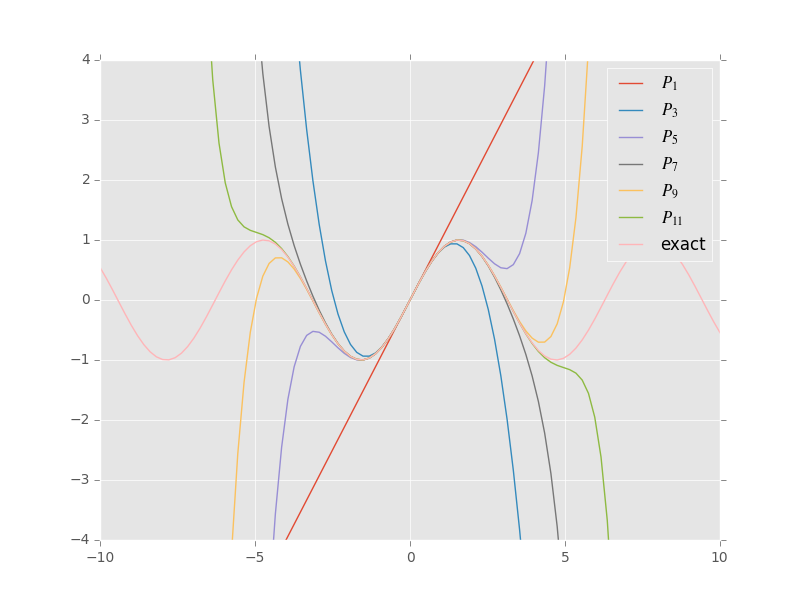
\includegraphics [height=3.5in]{taylor/taylor.eps}

    \end{center} \end{figure}%
\lthtmlfigureZ
\hfill\lthtmlcheckvsize\clearpage}

\stepcounter{subsection}
{\newpage\clearpage
\lthtmldisplayA{displaymath1210}%
\begin{displaymath}\pm 0.d_1 d_2 d_3 \ldots d_k \times 10^n,
\end{displaymath}%
\lthtmldisplayZ
\hfill\lthtmlcheckvsize\clearpage}

{\newpage\clearpage
\lthtmlinlinemathA{tex2html_wrap_inline1322}%
$0.64\times 10^7$%
\lthtmlinlinemathZ
\hfill\lthtmlcheckvsize\clearpage}

{\newpage\clearpage
\lthtmlinlinemathA{tex2html_wrap_inline1326}%
$-38 \leq n \leq 38$%
\lthtmlinlinemathZ
\hfill\lthtmlcheckvsize\clearpage}

{\newpage\clearpage
\lthtmlinlinemathA{tex2html_wrap_inline1328}%
$1.0\times
  10^{+38}$%
\lthtmlinlinemathZ
\hfill\lthtmlcheckvsize\clearpage}

{\newpage\clearpage
\lthtmlinlinemathA{tex2html_wrap_inline1330}%
$1.0\times 10^-38$%
\lthtmlinlinemathZ
\hfill\lthtmlcheckvsize\clearpage}

{\newpage\clearpage
\lthtmldisplayA{displaymath1211}%
\begin{displaymath}0.13391482 \times 10^5 \;\;\; {\rm and} \;\;\; 0.13391483 \times 10^5,
  \end{displaymath}%
\lthtmldisplayZ
\hfill\lthtmlcheckvsize\clearpage}

{\newpage\clearpage
\lthtmlinlinemathA{tex2html_wrap_inline1332}%
$0.13391482 \times 10^5$%
\lthtmlinlinemathZ
\hfill\lthtmlcheckvsize\clearpage}

{\newpage\clearpage
\lthtmlinlinemathA{tex2html_wrap_inline1342}%
$\times$%
\lthtmlinlinemathZ
\hfill\lthtmlcheckvsize\clearpage}

{\newpage\clearpage
\lthtmlfigureA{figure1148}%
\begin{figure}
    \begin{center}
      \leavevmode
      \htmlimage{scale=1.5}
      
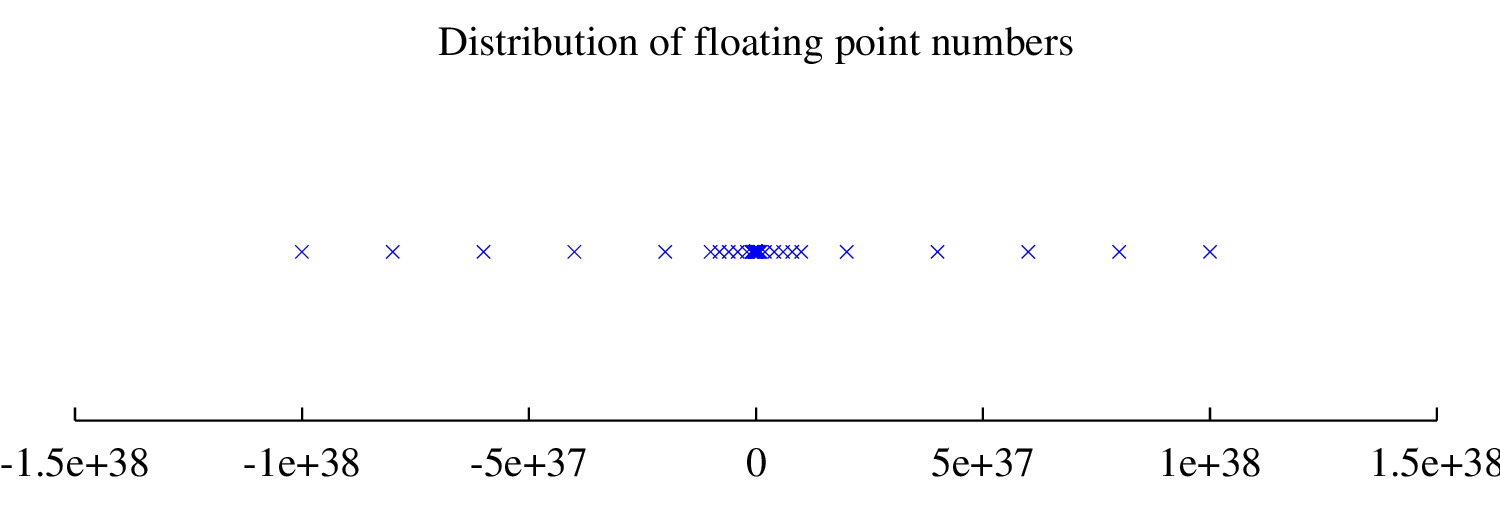
\includegraphics [width=5.0in]{float/float1.eps}
    \end{center}
  \end{figure}%
\lthtmlfigureZ
\hfill\lthtmlcheckvsize\clearpage}

{\newpage\clearpage
\lthtmlinlinemathA{tex2html_wrap_inline1352}%
$-308\leq n \leq 308$%
\lthtmlinlinemathZ
\hfill\lthtmlcheckvsize\clearpage}


\end{document}
